\clearpage
\subsection{Множество Мандельброта}
\label{Mandelbrot_demo}

\epigraph{You know, if you magnify the coastline, it still looks like
a coastline, and a lot of other things have this property. Nature has
recursive algorithms that it uses to generate clouds and Swiss cheese
and things like that.}
{Дональд Кнут, интервью (1993)}

Множество Мандельброта это фрактал, характерное свойство которого это самоподобие.

При увеличении картинки, вы видите, что этот характерный узор повторяется бесконечно.


Вот демо\footnote{Можно скачать \href{http://go.yurichev.com/17306}
{здесь},} 
написанное автором по имени \q{Sir\_Lagsalot} \InENRU 2009, 
рисующее множество Мандельброта, и это программа для x86 с размером файла всего 64 байта.
Там только 30 16-битных x86-инструкций.

Вот что она рисует:

\begin{figure}[H]
\centering
\myincludegraphics{examples/demos/mandelbrot/1.png}
\end{figure}

Попробуем разобраться, как она работает.

\subsubsection{Теория}

\myparagraph{Немного о комплексных числах}

Комплексное число состоит из двух чисел (вещественная (Re) и мнимая (Im).

Комплексная плоскость\EMDASH{}это двухмерная плоскость, где любое комплексное число может быть расположено:
вещественная часть\EMDASH{}это одна координата и мнимая --- вторая.

Некоторые базовые правила, которые нам понадобятся:

\begin{itemize}
\item Сложение: $(a+bi) + (c+di) = (a+c) + (b+d)i$

Другими словами:

$\operatorname{Re}(sum) = \operatorname{Re}(a) + \operatorname{Re}(b)$

$\operatorname{Im}(sum) = \operatorname{Im}(a) + \operatorname{Im}(b)$

\item Умножение: $(a+bi) (c+di) = (ac-bd) + (bc+ad)i$

Другими словами:

$\operatorname{Re}(product) = \operatorname{Re}(a) \cdot \operatorname{Re}(c) - \operatorname{Re}(b) \cdot \operatorname{Re}(d)$

$\operatorname{Im}(product) = \operatorname{Im}(b) \cdot \operatorname{Im}(c) + \operatorname{Im}(a) \cdot \operatorname{Im}(d)$

\item Возведение в квадрат: $(a+bi)^2 = (a+bi) (a+bi) = (a^2-b^2) + (2ab)i$

Другими словами:

$\operatorname{Re}(square) = \operatorname{Re}(a)^2-\operatorname{Im}(a)^2$

$\operatorname{Im}(square) = 2 \cdot \operatorname{Re}(a) \cdot \operatorname{Im}(a)$

\end{itemize}

\myparagraph{Как нарисовать множество Мандельброта}

Множество Мандельброта\EMDASH{}это набор точек, для которых рекурсивное соотношение
 $z_{n+1} = {z_n}^2 + c$ 
(где $z$ \AndENRU $c$ это комплексные числа и $c$ 
это начальное значение)
не стремится к бесконечности.\\
\\
Простым русским языком: 

\begin{itemize}
\item Перечисляем все точки на экране. 
\item Проверяем, является ли эта точка в множестве Мандельброта.
\item Вот как проверить:

  \begin{itemize}
  \item Представим точку как комплексное число.
  \item Возведем в квадрат.
  \item Прибавим значение точки в самом начале.
  \item Вышло за пределы? Прерываемся, если да.
  \item Передвигаем точку в новое место, координаты которого только что вычислили.
  \item Повторять всё это некое разумное количество итераций.
  \end{itemize}

\item Двигающаяся точка в итоге не вышла за пределы?
Тогда рисуем точку.

\item Двигающаяся точка в итоге вышла за пределы?

  \begin{itemize}
    \item (Для черно-белого изображения) ничего не рисуем.
    \item 
(Для цветного изображения) преобразуем количество итераций в какой-нибудь цвет.
Так что цвет будет показывать, с какой скоростью точка вышла за пределы.

  \end{itemize}

\end{itemize}

Вот алгоритмы для комплексных и обычных целочисленных чисел (на языке, отдаленно напоминающем Python):%


\lstinputlisting[caption=Для комплексных чисел]{examples/demos/mandelbrot/algo_cplx_RU.lst}

Целочисленная версия, это версия где все операции над комплексными числами заменены на операции 
с целочисленными, в соответствии с изложенными ранее правилами.


\lstinputlisting[caption=Для целочисленных чисел]{examples/demos/mandelbrot/algo_int_RU.lst}

Вот также исходный текст на C\#, который есть в статье в Wikipedia\footnote{\href{http://go.yurichev.com/17307}{wikipedia}}, но мы немного изменим его,
чтобы он выдавал количество итераций, вместо некоторого символа
\footnote{Здесь также и исполняемый файл: 
\href{http://go.yurichev.com/17163}{beginners.re}}:

\lstinputlisting{examples/demos/mandelbrot/dump_iterations.cs}

Вот файл с результатом, который слишком широкий, чтобы привести его здесь: \\
\href{http://go.yurichev.com/17164}{beginners.re}.

Максимальное число итераций 40, так что если вы видите 40 в этом файле, это означает что точка ходила
40 итераций, но так и не вышла за пределы.
 
Номер $n$ меньше 40 означает что эта точка оставалась внутри пределов только $n$ итераций, и затем
вышла наружу.


\clearpage
Вот здесь есть неплохая демонстрация: 
\url{http://go.yurichev.com/17309}, она показывает визуально,
как определенная точка двигается по плоскости на каждой итерации. 
Вот два скриншота.

В начале кликаем внутри желтой области, и увидим траекторию (зеленые линии), которая в итоге
загручивается в какой-то точке внутри:%


\begin{figure}[H]
\centering
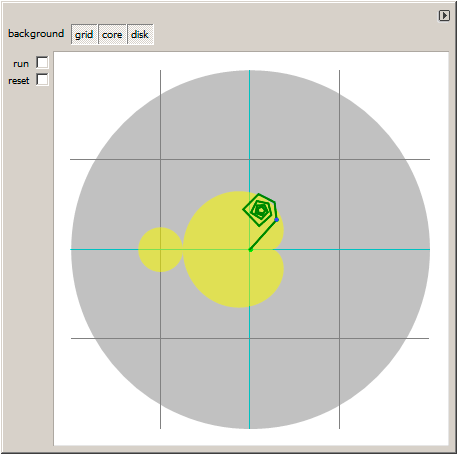
\includegraphics[width=0.7\textwidth]{examples/demos/mandelbrot/demo1.png}
\caption{Клик внутри желтой области}
\end{figure}

Это значит, что точка на которой кликнули, находится внутри множества Мандельброта.


\clearpage
Затем кликаем снаружи желтой области, и мы видим более хаотичные движения точки, которая быстро выходит
за пределы:


\begin{figure}[H]
\centering
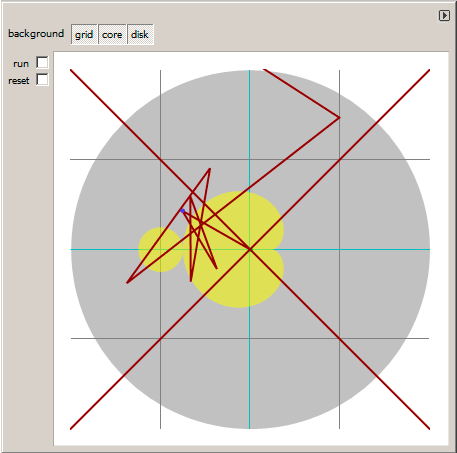
\includegraphics[width=0.7\textwidth]{examples/demos/mandelbrot/demo2.png}
\caption{Клик снаружи желтой области}
\end{figure}

Это значит, что эта точка не принадлежит множеству Мандельброта.

Другая неплохая демонстрация там: 
\url{http://go.yurichev.com/17310}.

\clearpage
\subsubsection{Вернемся к демо}

Демо, хотя и крошечная (только 64 байта или 30 инструкций), реализует общий алгоритм, изложенный
здесь, но с некоторыми трюками.


Исходный код можно скачать, так что вот он, но также снабдим его своими комментариями:

\lstinputlisting[caption=Исходный код с комментариями,numbers=left]{examples/demos/mandelbrot/Microbrot_commented_RU.asm}

Алгоритм:

\begin{itemize}
\item Переключаемся в режим VGA 320*200 256 цветов. 
$320*200=64000$ (0xFA00). 
Каждый пиксель кодируется одним байтом, так что размер буфера 0xFA00 байт.

Он адресуется здесь при помощи пары регистров ES:DI.

\myindex{x86!\Registers!ES}
ES должен быть здесь 0xA000, потому что это сегментный адрес видеобуфера, но запись
числа 0xA000 в ES потрубет по крайней мере 4 байта (\TT{PUSH 0A000h / POP ES}). 
О 16-битной модели памяти в MS-DOS, читайте больше тут: 
\myref{8086_memory_model}.

\myindex{x86!\Instructions!LES}
Учитывая, что BX здесь 0, и Program Segment Prefix находится по нулевому адресу, 2-байтная инструкция
\TT{LES AX,[BX]} запишет 0x20CD в AX и 0x9FFF в ES.

Так что программа начнет рисовать на 16 пикселей (или байт) перед видеобуфером.

Но это MS-DOS, 
здесь нет защиты памяти, так что запись происходит в самый конец обычной памяти, а там, как правило, ничего важного нет.

Вот почему вы видите красную полосу шириной 16 пикселей справа.
Вся картинка сдвинута налево на 16 пикселей.
Это цена экономии 2-х байт.

\item Вечный цикл, обрабатывающий каждый пиксель.
Наверное, самый общий метод обойти все точки на экране это два цикла:
один для X-координаты, второй для Y-координаты.

Но тогда вам придется перемножать координаты для поиска байта в видеобуфере VGA.
Автор этого демо решил сделать наоборот: перебирать все байты в видеобуфере при помощи одного цикла
вместо двух и затем получать координаты текущей точки при помощи деления.

В итоге координаты такие: X в пределах $-256..63$ \AndENRU Y 
в пределах $-100..99$.
Вы можете увидеть на скриншоте что картинка как бы сдвинута в правую часть экрана.
Это потому что самая большая черная дыра в форме сердца обычно появляется на координатах 0,0 и они
здесь сдвинуты вправо.

Мог ли автор просто отнять 160 от X, чтобы получилось значение в пределах $-160..159$? 
Да, но инструкция \TT{SUB DX, 160} занимает 4 байта, 
тогда как \TT{DEC DH}\EMDASH{}2 байта 
(которая отнимает 0x100 (256) от DX). 
Так что картинка сдвинута ценой экономии еще 2-х байт.

    \begin{itemize}
    \item Проверить, является ли текущая точка внутри множества Мандельброта.
          Алгоритм такой же, как и описанный здесь.
\myindex{x86!\Instructions!LOOP}
     \item Цикл организуется инструкцией \TT{LOOP}, которая использует регистр CX как счетчик.
Автор мог бы установить число итераций на какое-то число, но не сделал этого: потому что 320 уже
находится в CX (было установлено на строке 35), и это итак подходящее число как число максимальных
итераций.

Мы здесь экономим немного места, не загружая другое значение в регистр CX.

\myindex{x86!\Instructions!SAR}
     \item Здесь используется \TT{IMUL} вместо \TT{MUL}, потому что мы работаем с знаковыми значениями:
помните, что координаты 0,0 должны быть где-то рядом с центром экрана.

Тоже самое и с \TT{SAR} (арифметический сдвиг для знаковых значений): она используется вместо \TT{SHR}.


     \item Еще одна идея\EMDASH{}это упростить проверку пределов.
Нам бы пришлось проверять пару координат, т.е. две переменных.
Что делает автор это трижды проверяет на переполнение: две операции возведения в квадрат и одно 
прибавление.
Действительно, мы ведь используем 16-битные регистры, содержащие знаковые значения в пределах
 -32768..32767, так что
если любая из координат больше чем 32767 в процессе умножения, точка однозначно вышла за пределы,
и мы переходим на метку \TT{MandelBreak}.


     \item Здесь также имеется деление на 64 (при помощи инструкции SAR). 64 задает масштаб.

Попробуйте увеличить значение и вы получите более увеличенную картинку, или уменьшить для
меньшей.


    \end{itemize}

\item Мы находимся на метке \TT{MandelBreak}, есть только две возможности
попасть сюда: 
цикл закончился с CX=0 (точка внутри множества Мандельброта
); или потому что произошло переполнение (CX все еще содержит 
какое-то значение).
Записываем 8-битную часть CX (CL) в видеобуфер.
Палитра по умолчанию грубая, тем не менее, 0 это черный: поэтому видим черные дыры в местах где точки
внутри множества Мандельброта.

Палитру можно инициализировать в начале программы, но не забывайте, это всего лишь программа на 64 
байта!

\item Программа работает в вечном цикле, потому что дополнительная проверка, где остановится, 
или пользовательский интерфейс, это дополнительные инструкции.

\end{itemize}

Еще оптимизационные трюки:

\myindex{x86!\Instructions!CWD}
\begin{itemize}
\item 1-байтная CWD используется здесь для обнуления DX вместо двухбайтной \TT{XOR DX, DX} или даже трехбайтной \TT{MOV DX, 0}.

\item 1-байтная \TT{XCHG AX, CX} используется вместо двухбайтной 
\TT{MOV AX,CX}. 
Текущее значение в AX все равно уже не нужно.

\item DI (позиция в видеобуфере) не инициализирована, и будет 0xFFFE в
начале
\footnote{Больше о состояниях регистров на старте: 
\url{http://go.yurichev.com/17004}}.
Это нормально, потому что программа работает бесконечно для всех DI в пределах 0..0xFFFF, и пользователь
не может увидеть, что работала началась за экраном (последний пиксель видеобуфера 320*200 имеет адрес 0xF9FF).

Так что некоторая часть работы на самом деле происходит за экраном.
А иначе понадобятся дополнительные инструкции для установки DI в 0; добавить проверку на конец буфера.


\end{itemize}

\newcommand{\MyFixedVersion}{Моя \q{исправленная} версия}
\subsubsection{\MyFixedVersion}

\lstinputlisting[caption=\MyFixedVersion,numbers=left]{examples/demos/mandelbrot/my_version_RU.asm}

Автор сих строк попытался исправить все эти странности: теперь палитра плавная черно-белая, видеобуфер на правильном месте
(строки 19..20), картинка рисуется в центре экрана (строка 30), программа в итоге заканчивается и ждет,
пока пользователь нажмет какую-нибудь клавишу (строки 58..68).

Но теперь она намного больше: 105 байт (или 54 инструкции)

\footnote{Можете поэкспериментировать и сами: скачайте DosBox и NASM и компилируйте так:
 
\TT{nasm fiole.asm -fbin -o file.com}}.

\begin{figure}[H]
\centering
\myincludegraphics{examples/demos/mandelbrot/fixed.png}
\caption{\MyFixedVersion}
\label{fig:mandelbrot_fixed}
\end{figure}
